\documentclass[a4paper,11pt,uplatex]{jsarticle}
\usepackage{amsmath,amssymb}
\usepackage{bm}
\usepackage[dvipdfmx]{graphicx}
\usepackage{here}
\usepackage{longtable}

%テキストの表示領域の調節
\setlength{\textwidth}{\paperwidth}
\addtolength{\textwidth}{-40truemm}
\setlength{\textheight}{\paperheight}
\addtolength{\textheight}{-45truemm}

%余白の調節
\setlength{\topmargin}{-10.4truemm}
\setlength{\evensidemargin}{-5.4truemm}
\setlength{\oddsidemargin}{-5.4truemm}
\setlength{\headheight}{17pt}
\setlength{\headsep}{10mm}
\addtolength{\headsep}{-17pt}
\setlength{\footskip}{5mm}

\title{12.風洞実験}
\author{Ⅲ類機械システムプログラム 1610004 青木良太}
\date{提出日 2019年1月17日}
% \nofiles
\begin{document}
\maketitle
\section{目的}
現象の観察は,その現象を理解する上で最も基本的な行為である.特に流体現象は身近に存在しているため,古くから観察の対象となっていた.
流体現象を実験室で再現する装置の一つに風洞があり,電子計算機の発達に大きく貢献している.電子計算機の発達によってコンピュータ支援設計(CAD)が主流となった現在でも,
設計した機器の性能は実験を行うことでのみ確認される.
\par
本実験では,2次元小型煙風洞を用いて実験を行い,講義で学んだ原理・理論を実現象によって確認するとともに,流速と圧力の関係の測定や流れの可視化により流体力学的基礎事項を体験する.
\section{原理}
風洞実験は航空機や列車,自動車の設計には欠かせないものであるが,実寸大の模型で実験を行うことは困難であるため,縮小模型を用いることが多い.
では,縮小模型を用いた実験結果と実寸大の物体周りの現象が一致する原理について考える.
\subsection{Navier-Stokes方程式とレイノルズの相似則}
2次元流れ場において流体の圧縮性が無視でき,流体に外力が作用していない場合,Navier-Stokes方程式は次式で表される.
\begin{align}
  \rho \left( \frac{\partial u}{\partial t} + u\frac{\partial u}{\partial x} + v\frac{\partial u}{\partial y} \right) &= -\frac{\partial p}{\partial x} + \mu \left( \frac{\partial^2 u}{\partial x^2} + \frac{\partial^2 u}{\partial y^2} \right) \\
  \rho \left( \frac{\partial v}{\partial t} + u\frac{\partial v}{\partial x} + v\frac{\partial v}{\partial y} \right) &= -\frac{\partial p}{\partial y} + \mu \left( \frac{\partial^2 v}{\partial x^2} + \frac{\partial^2 v}{\partial y^2} \right)
\end{align}
ここで,$t$は時間,$(x,y)$は空間座標,$(u,v)$は流速の$(x,y)$方向成分,$p$は圧力,$\rho$は密度,$\mu$は粘性率である.
左辺は流体の慣性力,右辺第1項は圧力勾配,右辺第2項は粘性力を示しており,粘性力と慣性力が無視できない場合,これら二つの力の関係によって流れ場は左右される.
そこで,慣性力と粘性力の比をレイノルズ数Reとする.流れ場における代表的な速度を$U$,代表的な長さを$L$とすると,レイノルズ数は以下の式で表される.
\begin{align}
  \label{レイノルズ数}
  \mathrm{Re} = \frac{\mbox{慣性力}}{\mbox{粘性力}} = \frac{\mbox{質量} \times \mbox{加速度}}{\mbox{剪断応力} \times \mbox{面積}} = \frac{\rho L^3 \times \frac{U}{L/U}}{\mu \frac{U}{L} \times L^2} = \frac{UL}{\nu}
\end{align}
$\nu$は動粘性率である.
\par
図\ref{レイノルズ}のような幾何学的に相似な2つの流れに幾何学的に相似な物体を置く場合を考える.\cite{s2}これらはスケールこそ違うものの,流れのレイノルズ数が等しく,慣性力と粘性力の比が等しいため,力学的に相似であるといえる.
幾何学的・力学的に相似である2つの流れでは,一方の流れの様子や,物体に作用する力を確認し,それぞれ幾何学的,力学的倍率をかけることで他方の流れの様子が得られる.
これをレイノルズの相似則といい,この法則を用いることで,縮小模型による流れの実験から大きなスケールの事象を確認することができる.


\begin{figure}[H]
  \begin{center}
    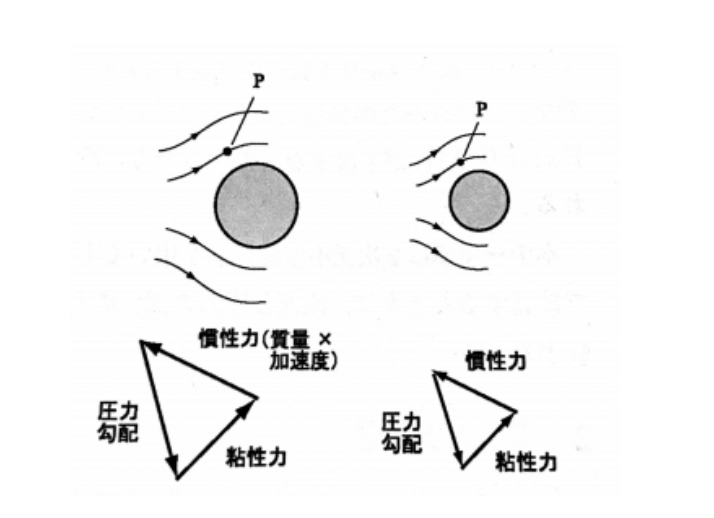
\includegraphics[width = 7cm]{pic/reinolz.png}
    \caption{レイノルズ相似}
    \label{レイノルズ}
  \end{center}
\end{figure}
\subsection{円柱周りの流れ\cite{s3}}
レイノルズ数に応じて流れの様子が変化する流れの代表的なものとして,直径$d$の円柱を過ぎる一様流(速さ$U$)が挙げられる.
図\ref{図2:変化}に円柱周りの流れの様子を,図\ref{抗力変化}に円柱に作用する抗力の$Re(=Ud/\nu)$に対する変化を示す.
図\ref{抗力変化}中のアルファベットが示すレイノルズ数領域は,図\ref{図2:変化}の副番号と対応している.


\begin{figure}[H]
  \begin{center}
    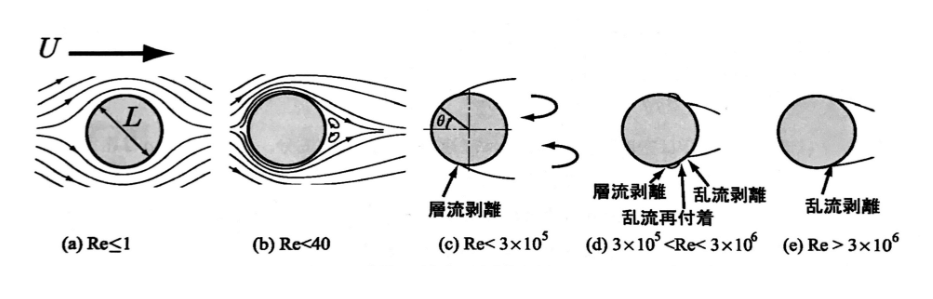
\includegraphics[width = 10cm]{pic/流れの変化.png}
    \caption{レイノルズ数に対する円柱周りの流れの変化\cite{s3}}
    \label{図2:変化}
  \end{center}
\end{figure}
\begin{figure}[H]
  \begin{center}
    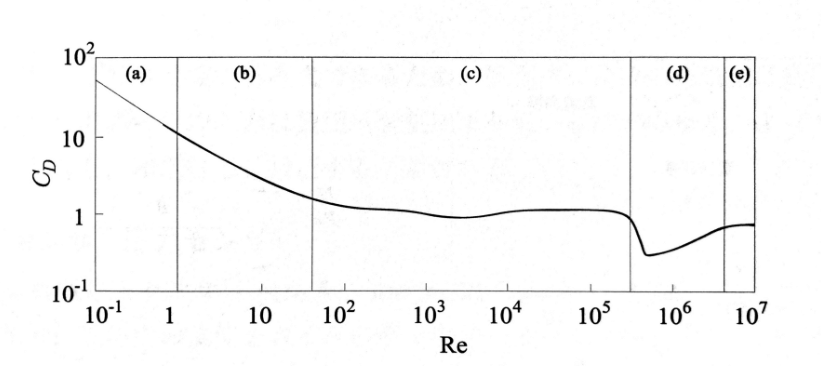
\includegraphics[width = 10cm]{pic/抗力.png}
    \caption{円柱に作用するレイノルズ数に対する変化\cite{s3}}
    \label{抗力変化}
  \end{center}
\end{figure}

\newpage
Re$\leq$1の時では,流体は図2の(a)のように円柱に沿って流れ,剥離をしない.流れ破堤上流であり,一両流の方向に対して円柱中心から上下対称かつ前後対称となる.$2\leq$Re$\leq40$になると,円柱後流には双子渦と呼ばれる一対の渦が生じる.この双子渦はレイノルズ数の増加に従っって下流側に成長する.レイノルズ数が増加する(Re$\leq10^2$)と渦が振動し始め,円柱から渦が交互に放出される非定常な流れとなる.円柱下流ではカルマン渦列が形成され,カルマン渦はRe<$10^3$で3次元的になり,単一性の周期は消滅する.しかしながら,$10^2$<Re$\leq 3 \times 10^5$になると,レイノルズ数が増加しても剥離点は$\theta = 80$度付近ではほとんど変化せず,円柱に作用する抗力係数は一定となる.Re $ =3 \times 10^5$ 付近になると,円柱表面の境界層が乱流に遷移して,図\ref{図2:変化}のように剥離点は135$^\circ$付近まで後退していく.この時抗力係数は0.3以下に減少し,この時のレイノルズ数を臨界レイノルズ数と呼ぶ.つまり,層流から乱流にへと遷移する時の境界の値が臨界レイノルズ数である.この値よりもレイノルズ数が増加すると剥離点は前方に移動し,抗力係数は増加する.
\par
次に,前縁淀み点からの角度を$\theta$とすると,異なるレイノルズ数における円柱周りの圧力分布は図\ref{円柱周りの圧力}のようになる.円柱周りの圧力分布はレイノルズ数によって大きく変化しており,特に臨界レイノルズ数前後での変化が大きいことがわかる.
\par
式(\ref{レイノルズ数})によると,Reが大きい流体では慣性力に対して,粘性力が与える影響は小さいため,粘性を考えない非粘性流体として考えることができる.
この流れはポテンシャル流(渦なし流)の理論によって扱うことでき,前縁淀み展からの角度$\theta$と円柱表面上の速度$v_{\theta}$を図\ref{ポテンシャル流れ}のようにとると,円柱表面の任意の点における流速$v_{\theta}$は次のように表される.\cite{s4}:
\begin{align}
  v_{\theta} = 2U\sin \theta
\end{align}

\begin{figure}[H]
  \begin{center}
    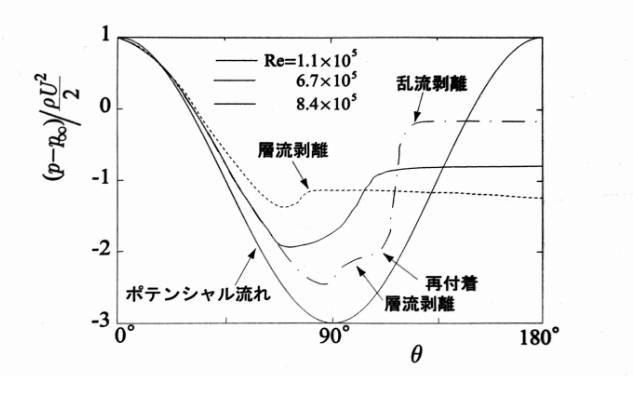
\includegraphics[width = 10cm]{pic/円柱周りの圧力.png}
    \caption{円柱周りの圧力分布\cite{s4}}
    \label{円柱周りの圧力}
  \end{center}
\end{figure}
\begin{figure}[H]
  \begin{center}
    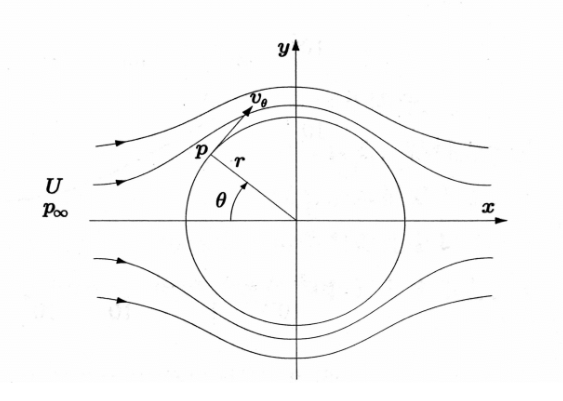
\includegraphics[width = 10cm]{pic/円柱周りのポテンシャル.png}
    \caption{円柱周りのポテンシャル流れ\cite{s4}}
    \label{ポテンシャル流れ}
  \end{center}
\end{figure}

また,一様流中の圧力を$p_{\infty}$,円柱表面の任意の点における圧力を$p$とすると,ベルヌーイの定理より,次式が得られる.
\begin{align}
  \label{ポテンシャル式}
  p - p_{\infty} = \frac{\rho U^2}{2}(1 - 4 \sin^2 \theta)
\end{align}
図\ref{円柱周りの圧力}には式(\ref{ポテンシャル式})によって示される円柱周りの圧力分布も表されている.ポテンシャル流による圧力は$\theta = 90^{\circ}$を軸として対象に分布しており,実際の圧力分布とかなり異なっている(特に円柱後方で差異が著しい).

\section{実験方法}
\subsection{実験装置}
\subsubsection{2次元小型煙風洞}
  実験で使用した風洞は,西日本流体技研製のST-30Aである.その概略図を図\ref{風洞図}に示す.風洞の流速はインバータモータによって調整するが,風洞には流速を表示する機能はないため,インバータ駆動時の出力電圧をデジタルマルチメータ(ADVENTEST製,R6441B)を用いて測定した.
  また,流速計(SIBATA製,WIND BOY ISA-80)を用いて流速を測定し,インバータ電圧と流速の関係を求めた.
  \par
  また,本実験では吸い込み式で測定したため,風洞内に流入した空気は動圧に相当する圧力降下を受けるため,風洞内の平均圧力は負圧となった.そこで,測定した圧力に動圧分を加算し,測定結果を補正した.

  \begin{figure}[H]
    \begin{center}
      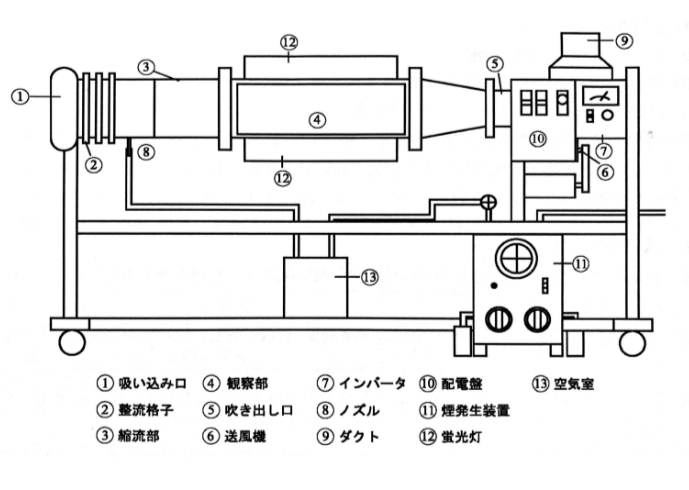
\includegraphics[width = 10cm]{pic/風洞図.png}
      \caption{風洞の概略図}
      \label{風洞図}
    \end{center}
  \end{figure}
\subsubsection{微差圧センサ}
圧力の測定には微差圧センサ(setra製,model 267)を用いた.微差圧センサは可変リアクタンス式であり,受圧面の変位をコイルの容量変化により電気的に検出した.センサ定格は$\pm$250Paであり,測定された圧力の値はセンサに設けられた液晶画面に表示された.なお,微差圧センサは単体では駆動できないため,直流安定化電源(METRONIX製 MODEL 544A)より電源を供給した.なお,微差圧センサは過負荷に対して脆弱であるため,実験中は供試模型と圧力センサを接続するチューブに過度の負荷を与えないように注意した.
\subsubsection{煙発生装置}
流れの可視化には,煙発生装置(ツクバリカセイキ製,F-235)を用いた.
煙発生装置ないのニクロム線に電圧をかけて発熱させ,油を滴下することにより煙を発生させた.煙は送風機により,空気しつを経由して櫛状ノズルより風洞内へと導かれる.発煙用油として,発生する煙が無害なオンジナオイルを用いた.
可視化した流れはデジタルカメラ(Canon製,EF-S 18-55 IS)により記録した.
\subsubsection{供試模型}
定点での圧力測定および円柱の圧力分布測定には,圧力孔の設けられた円柱を用いる.表1に可視化実験で用いる供試模型の代表長さを示す.また,図に実験に用いた翼および自動車の模型の断面を示す.翼をJoukowski変換によって円を写像したJoukowski翼であり,航空機に用いられる翼とは異なる.自動車はプリメーラP11型(日産自動車,1995 2001年製造)を参考に作成した.
\begin{table}[H]
  \centering
  \caption{可視化実験に用いる供試模型の形状と代表長さ}
  \label{供試模型}
  \begin{tabular}{ccccc} \hline
  供試模型 & 円柱 & 正四角柱 & 翼 & 自動車  \\ \hline
   代表長さ $L$[mm]&34(直径)& 40(一辺長)& 99(翼弦長)& 136(車長) \\ \hline
  \end{tabular}
\end{table}

\begin{figure}[H]
  \centering
  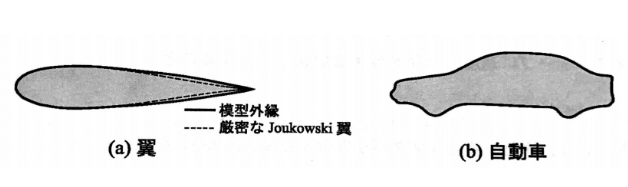
\includegraphics[width =10cm]{pic/断面.png}
  \caption{供試模型断面}
  \label{断面}
\end{figure}

\subsection{実験手順}
\subsubsection{風洞検定実験}
風洞検定実験では,3.1節に示した実験装置のうち,2次元小型煙風洞,デジタルマルチメータ(インバータ駆動時の電圧出力用流速)
を用いた.実験手順を以下に示す.
\begin{enumerate}
  \item 風洞測定部の背面が流速測定用の背板になっていること,排煙ダクトを取り外した状態であることを確認した.
  \item 風洞測定部の上部に設置された蛍光灯を取り外し,流速計を測定部中央に挿入した.
  \item インバータ電圧を0.010Vから0.080Vまで0.005Vずつ上昇させ,流速計を用いて流速を測定した.
  \item 測定した流速を順次グラフ用紙にプロットし,測定終了後に近似直線を引いた.以降の実験では作成した図に基づいてインバータ電圧を流速に換算した.なお,インバータの特性により,低電圧時にはインバータ電圧とファン回転数に線形関係が得られない.そのため,近似直線はインバータ電圧0V時に流速0m/sを通過しないことに注意する.
\end{enumerate}
\subsubsection{定点での圧力測定}
\begin{enumerate}
  \item 風洞測定部の背板を,圧力測定用に交換した.
  \item 微差圧センサの駆動用電源が切れていることを確認し,圧力測定用円柱に取り付けられたゴムチューブを微差圧センサに接続した.
  \item 円柱に設けられた圧力孔を0$^\circ$,45$^\circ$,90$^\circ$,135$^\circ$,180$^\circ$の各位置に固定し,流速を次第に増加させた時の圧力と流速の関係を調べた.
  \item 測定後,微差圧センサの駆動用電源を切った.
\end{enumerate}

\subsubsection{円柱周りの圧力分布の測定}
\begin{enumerate}
  \item 流速を一定とし,圧力測定孔を0$^\circ$から345$^\circ$まで,15$^\circ$刻みで回転させ,円柱表面の圧力分布を測定した.345$^\circ$まで測定した後,円柱を測定時に回転させた方向とは逆方向に回転させ,圧力測定孔を0$^\circ$に戻した.
  \item 流速を変更し,同様の手順を繰り返した.
  \item 測定が終了した後,微差圧センサ駆動用電源を切った.
\end{enumerate}

\subsubsection{流れの可視化}
\begin{enumerate}
  \item 可視化用の煙を室外に排出するため,排煙ダクトを取り付けた.また,実験室の換気扇が作動していると風洞内の流れに影響があるため,換気扇を止めた.
  \item 風洞測定部の背板を可視化実験用に交換した.供試模型には,円柱,正四角柱,翼,自動車を用いた.
  \item 表\ref{可視化実験}に示す実験方法に従って煙を流し,円柱,正四角柱,翼,自動車の順に流れを可視化し,流れの様子をデジタルカメラで撮影した.
\end{enumerate}

\begin{table}[H]
  \centering
  \caption{可視化実験方法}
  \label{可視化実験}
  \begin{tabular}{ccc} \hline
  供試模型 & 実験方法 & 観察点  \\ \hline
   \begin{tabular}{c} 円柱 \\ 自動車\end{tabular}
   & \begin{tabular}{c}模型を固定し,流速を変化させて \\ 流れの変化を観察する.\end{tabular}
   & \begin{tabular}{c}流速の変化に対する模型表面 \\ からの剥離位置や後流渦の変化 \end{tabular} \\ \hline

   \begin{tabular}{c} 正四角柱 \\ 翼 \end{tabular}
   &\begin{tabular}{c} 流速を固定し,模型の迎え角を \\ 変化させて流れの変化を観察する.\end{tabular}
   &\begin{tabular}{c} 模型仰角の変化に対する \\ 剥離位置や後流渦の変化 \end{tabular} \\ \hline
   \end{tabular}
\end{table}

\section{実験結果及び考察}
\subsection{風洞検定実験}
風洞実験より求められた,インバータ電圧$E_R$と流速$U_R$との関係を図\ref{インバータ電圧と流速}に示す.

\begin{figure}[H]
  \begin{center}
    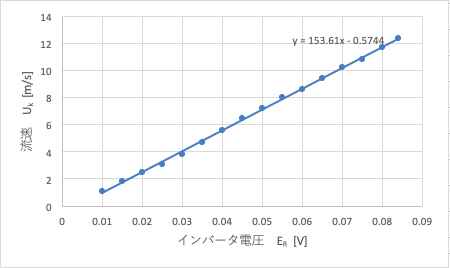
\includegraphics[width = 10cm]{pic/インバータと流速.png}
    \caption{インバータ電圧と流速の関係}
    \label{インバータ電圧と流速}
  \end{center}
\end{figure}

図\ref{インバータ電圧と流速}を見ると,インバータ電圧$E_R$と流速$U_R$は線形の相関があることがわかる.
また,この近似した一次関数が原点を通らないことは,インバータ電圧が低電圧の領域では線形ではなく,曲線の関係になることがわかる.

\subsection{定点での圧力測定}
円柱の定点における圧力を測定した結果を表\ref{定点表}に示す.また,表\ref{定点表}をもとに作成した流速と圧力の関係を図\ref{定点測定}に示す.

\begin{longtable}{llll}
\caption{円柱の定点における圧力の測定結果} \label{定点表} \\
角度[$^\circ$] & 回転電圧 [V]& 流速 [m/s]& 圧力 [Pa] \\ \hline \hline
\endfirsthead
%------ 2ページ以降の表の最上部 ----
\multicolumn{4}{r}{前ページからの続き} \\ \hline
角度[$^\circ$] & 回転電圧 [V]& 流速 [m/s]& 圧力 [Pa]  \\ \hline\hline
\endhead
%----- ページの表の最下部 --------
\hline
\multicolumn{4}{r}{次ページに続く} \\
\endfoot
%----- 最終ページの表の最下部 --------
\hline
\multicolumn{4}{r}{以上} \\
\endlastfoot
0 & 0.01 & 0.9 & 0 \\ \cline{2-4}
 & 0.02 & 2.4 & -1 \\ \cline{2-4}
 & 0.03 & 4 & -2 \\ \cline{2-4}
 & 0.04 & 5.5 & -3 \\ \cline{2-4}
 & 0.05 & 7.1 & -4 \\ \cline{2-4}
 & 0.06 & 8.6 & -5 \\ \cline{2-4}
 & 0.07 & 10.2 & -7 \\ \cline{2-4}
 & 0.08 & 11.7 & -9 \\ \hline  \hline
45 & 0.01 & 0.90 & -1 \\ \cline{2-4}
 & 0.02 & 2.40 & -5 \\ \cline{2-4}
 & 0.03 & 4.00 & -12 \\ \cline{2-4}
 & 0.04 & 5.50 & -24 \\ \cline{2-4}
 & 0.05 & 7.10 & -39 \\ \cline{2-4}
 & 0.06 & 8.60 & -60 \\ \cline{2-4}
 & 0.07 & 10.20 & -82 \\ \cline{2-4}
 & 0.08 & 11.70 & -107 \\ \hline \hline
90 & 0.01 & 0.90 & -2 \\ \cline{2-4}
 & 0.02 & 2.40 & -8 \\ \cline{2-4}
 & 0.03 & 4.00 & -20 \\ \cline{2-4}
 & 0.04 & 5.50 & -38 \\ \cline{2-4}
 & 0.05 & 7.10 & -62 \\ \cline{2-4}
 & 0.06 & 8.60 & -91 \\ \cline{2-4}
 & 0.07 & 10.20 & -125 \\ \cline{2-4}
 & 0.08 & 11.70 & -168 \\ \hline \hline
135 & 0.01 & 0.90 & -1 \\ \cline{2-4}
 & 0.02 & 2.40 & -7 \\ \cline{2-4}
 & 0.03 & 4.00 & -20 \\ \cline{2-4}
 & 0.04 & 5.50 & -37 \\ \cline{2-4}
 & 0.05 & 7.10 & -62 \\ \cline{2-4}
 & 0.06 & 8.60 & -90 \\ \cline{2-4}
 & 0.07 & 10.20 & -123 \\ \cline{2-4}
 & 0.08 & 11.70 & -168 \\ \hline \hline
180 & 0.01 & 0.90 & -1 \\ \cline{2-4}
 & 0.02 & 2.40 & -7 \\ \cline{2-4}
 & 0.03 & 4.00 & -22 \\ \cline{2-4}
 & 0.04 & 5.50 & -41 \\ \cline{2-4}
 & 0.05 & 7.10 & -68 \\ \cline{2-4}
 & 0.06 & 8.60 & -103 \\ \cline{2-4}
 & 0.07 & 10.20 & -138 \\ \cline{2-4}
 & 0.08 & 11.70 & -190 \\ \cline{2-4}
\end{longtable}

\begin{figure}[H]
  \begin{center}
    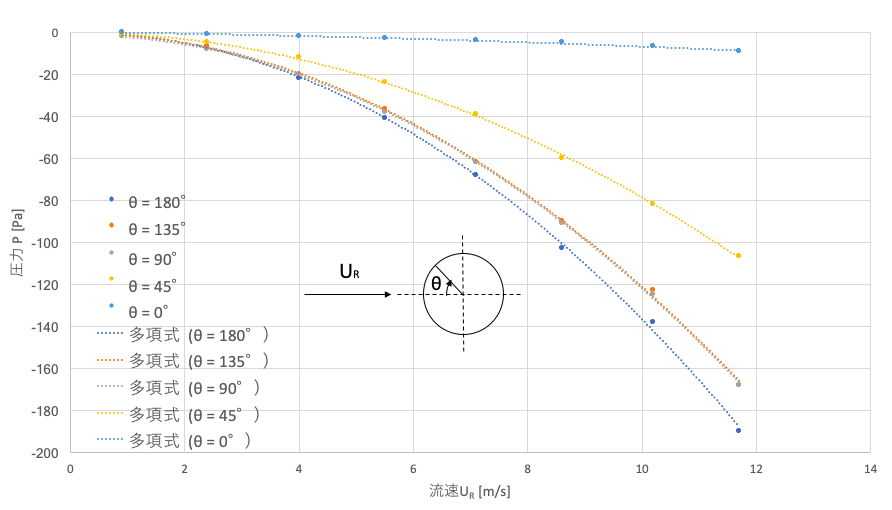
\includegraphics[width = 10cm]{pic/流速と圧力2.png}
    \caption{定点での圧力測定結果}
    \label{定点測定}
  \end{center}
\end{figure}

図\ref{定点測定}を見ると,常に負圧となっている.これは吸い込み式風洞において,動圧分だけ大気圧よりも低くなっているためである.また,$\theta$が0$^\circ$45$^\circ$までは流速が大きくなるにつれて負圧が大きくなっているが,$\theta $が$90^{\circ}$を越えると同じ軌跡を描いている.これは$90^{\circ}$付近で流れが剥離するために,角度による圧力の変化が小さいと思われる.

\subsection{円柱周りの圧力分布}
円柱回りの圧力測定結果から,圧力測定孔角度と圧力の関係およびその理論値を示す丸型グラフをインバータ電圧0.04[V],0.06[V],0.08[V],すなわち流速5.5[m/s],8.6[m/s],11.7[m/s]について作成した.作成した丸型グラフはそれぞれ図10,11,12としてレポート末尾に添付した.
また、理論値はポテンシャル理論に基づく円柱表面の圧力分布の式
\begin{align}
  p = \frac{1}{2} \rho U_{R}^{2}(1-4 \sin^{2} \theta)
\end{align}
から求め,点線で示した.丸型グラフを見ると、$ -15^{\circ} \leq \theta \leq 15^{\circ}$の範囲では測定値と理論値で似た値を取っているが、それ以外の点では測定値と理論値で大幅に差があるのが分かる。これは,理論値を求めるための式(6)において、流体の粘性の影響を考慮していないためと思われる。桑原[\cite{s5}]によると,完全流体中の等速運動をする物体には抵抗が働かない(ダランベールのパラドックス)とするパラドックスがあり,空気は粘性が小さいため完全流体とみなせるが,実際には抵抗が働くとしている.
また,圧力分布は$\theta = \pm90^{\circ}$以降ではほぼ一定の値をとっている.これは流れが剥離したために圧力が回復せず,圧力が一定になっている.


\setcounter{figure}{12}
\subsubsection{流れの可視化}
円柱周りの流れを可視化した結果を図\ref{1_1}〜\ref{1_3}として以下に示す.
\begin{figure}[H]
  \begin{tabular}{cc}
    \begin{minipage}{0.5\hsize}
      \centering
      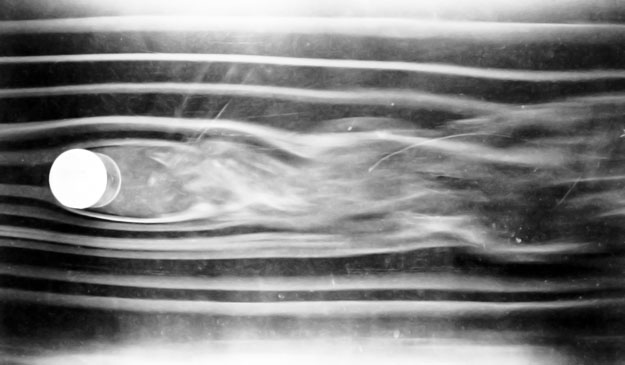
\includegraphics[width = 5cm]{pic/001.jpg}
      \caption{円柱周りの流れの可視化($E_R = 0.015[V]$)}
      \label{1_1}
    \end{minipage}

    \begin{minipage}{0.5\hsize}
      \centering
      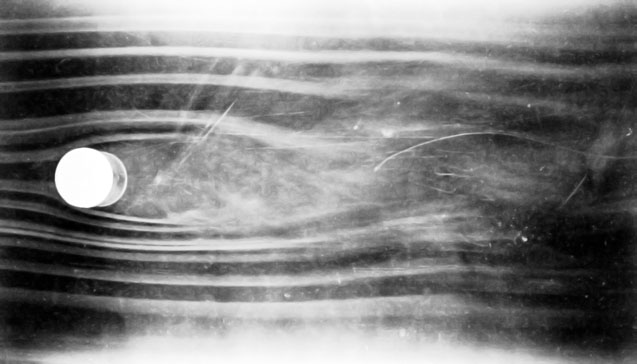
\includegraphics[width = 5cm]{pic/002.jpg}
      \caption{円柱周りの流れの可視化($E_R = 0.020[V]$)}
      \label{1_2}
    \end{minipage}
  \end{tabular}
\end{figure}

\begin{figure}[H]
  \begin{center}
    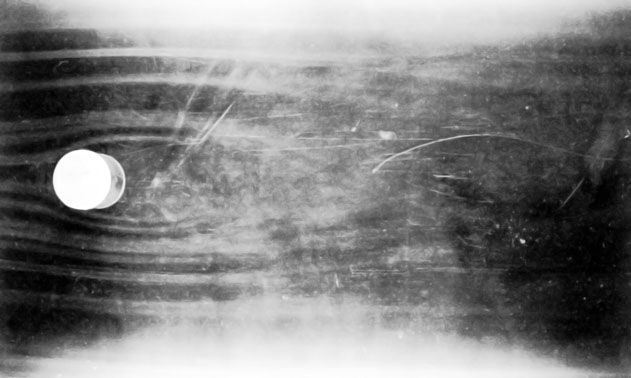
\includegraphics[width = 5cm]{pic/003.jpg}
    \caption{円柱周りの流れの可視化($E_R = 0.024[V]$)}
    \label{1_3}
  \end{center}
\end{figure}

図13〜15を比較すると,電圧が増加,すなわち流速が大きくなるほど流れが乱れているのが見て取れる.また,円柱の風下に見られるカルマン渦列も電圧が大きくなるほど顕著に現れているのが分かる。円柱ではおおよそ$\theta = 90^\circ$以降から流体の剥離が確認できる.
円柱の下流に煙が薄く広がった領域が見られ,速度の増加にしたがって薄くなっている.

次に自動車模型の流れを可視化した結果を図\ref{2_1}〜\ref{2_3}として以下に示す.
\begin{figure}[H]
  \begin{tabular}{cc}
    \begin{minipage}{0.5\hsize}
      \centering
      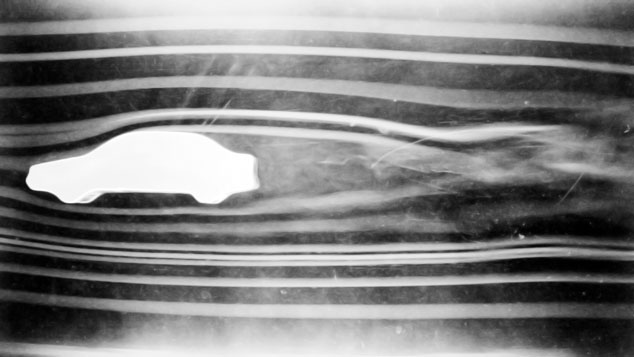
\includegraphics[width = 5cm]{pic/011.jpg}
      \caption{自動車模型の流れの可視化($E_R = 0.016[V]$)}
      \label{2_1}
    \end{minipage}

    \begin{minipage}{0.5\hsize}
      \centering
      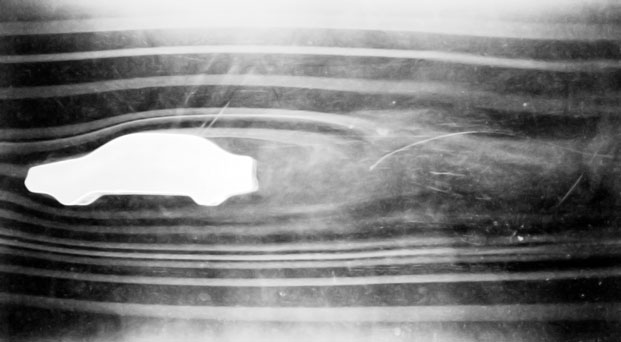
\includegraphics[width = 5cm]{pic/012.jpg}
      \caption{自動車模型の流れの可視化($E_R = 0.021[V]$)}
      \label{2_2}
    \end{minipage}
  \end{tabular}
\end{figure}

\begin{figure}[H]
  \begin{center}
    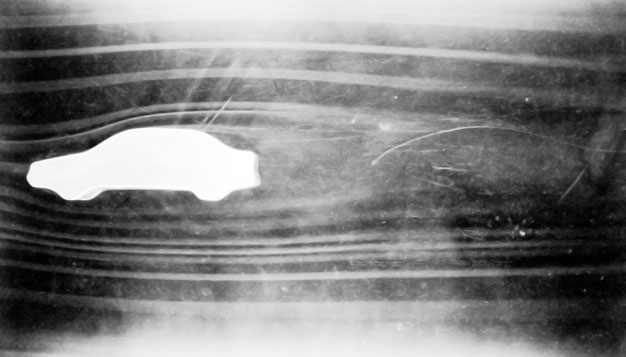
\includegraphics[width = 5cm]{pic/013.jpg}
    \caption{自動車模型の流れの可視化($E_R = 0.027[V]$)}
    \label{2_3}
  \end{center}
\end{figure}

車体の天井の終わりあたりから流れが剥離し始め、乱流が発生している。やはり電圧の大きさに応じて乱流が多く生じている。また発生しているカルマン渦列は円柱のものに比べて小さいように思われる。これは,自動車が円柱よりも流線型に近い形であるためである.円柱と違い,下流の薄い煙は速度が増加してもあまり変化は見られなかった.

続いて正四角柱の流れを可視化した結果を図\ref{3_1}〜\ref{3_3}として以下に示す.
\begin{figure}[H]
  \begin{tabular}{cc}
    \begin{minipage}{0.5\hsize}
      \centering
      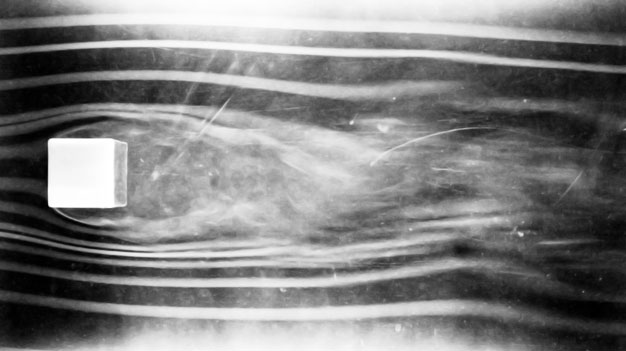
\includegraphics[width = 6cm]{pic/004.jpg}
      \caption{正四角柱の流れの可視化($\theta = 0 ^{\circ}$)}
      \label{3_1}
    \end{minipage}

    \begin{minipage}{0.5\hsize}
      \centering
      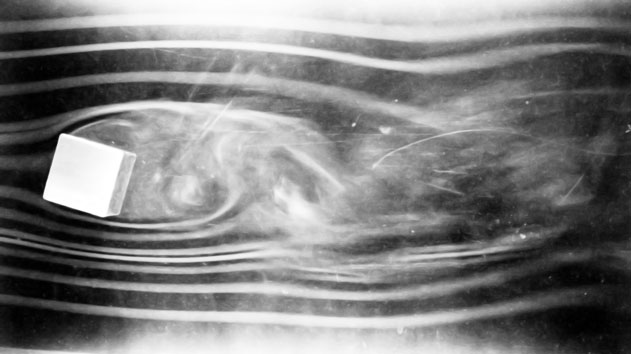
\includegraphics[width = 6cm]{pic/005.jpg}
      \caption{正四角柱の流れの可視化($\theta = 15 ^{\circ}$)}
      \label{3_2}
    \end{minipage}
  \end{tabular}
\end{figure}

\begin{figure}[H]
  \begin{center}
    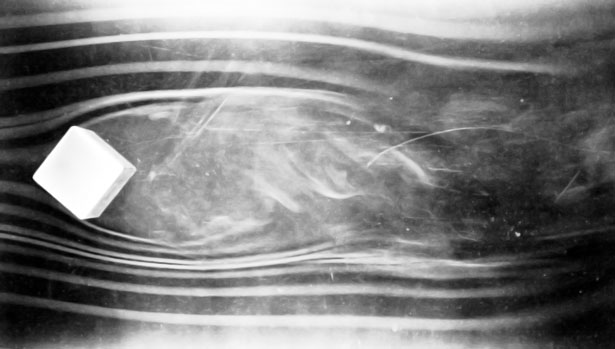
\includegraphics[width = 6cm]{pic/006.jpg}
    \caption{正四角柱の流れの可視化($\theta = 45 ^{\circ}$)}
    \label{3_3}
  \end{center}
\end{figure}

図より、正四角柱の場合では、迎え角$\theta$が$0^\circ$から$45^\circ$へと大きくなるにつれて流れの乱れ方や発生するカルマン渦列が大きくなっていることがよく分かる。いずれの角度においても四角柱の角で剥離しており,急激な形状の変化によって剥離がしやすくなることがわかる.
最後に,翼の模型の流れを可視化した結果を図\ref{4_1}〜\ref{4_4}として以下に示す.

\begin{figure}[H]
  \begin{tabular}{cc}
    \begin{minipage}{0.5\hsize}
      \centering
      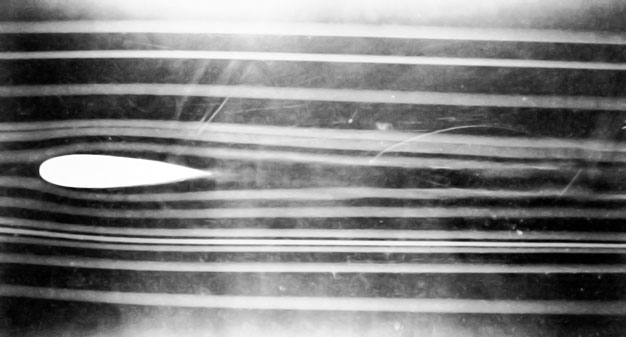
\includegraphics[width = 6cm]{pic/007.jpg}
      \caption{翼の模型の流れの可視化($\theta = 0 ^{\circ}$)}
      \label{4_1}
    \end{minipage}

    \begin{minipage}{0.5\hsize}
      \centering
      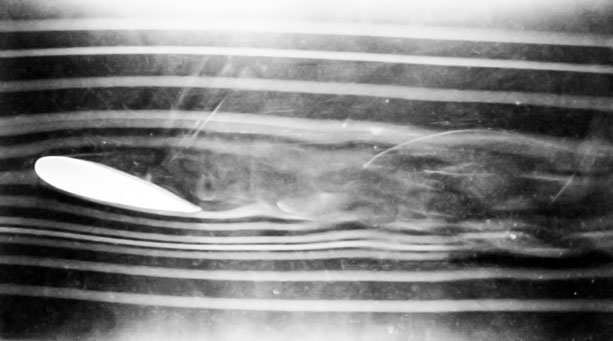
\includegraphics[width = 6cm]{pic/008.jpg}
      \caption{翼の模型の流れの可視化($\theta = 15 ^{\circ}$)}
      \label{4_2}
    \end{minipage}
  \end{tabular}
\end{figure}

\begin{figure}[H]
  \begin{tabular}{cc}
    \begin{minipage}{0.5\hsize}
      \centering
      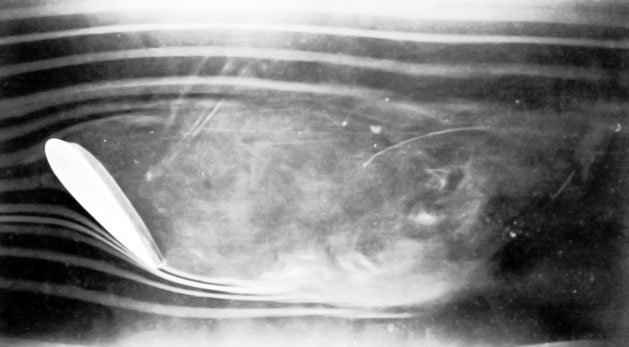
\includegraphics[width = 6cm]{pic/009.jpg}
      \caption{翼の模型の流れの可視化($\theta = 50 ^{\circ}$)}
      \label{4_3}
    \end{minipage}

    \begin{minipage}{0.5\hsize}
      \centering
      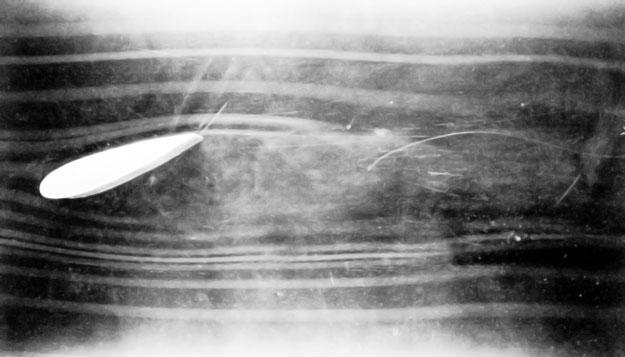
\includegraphics[width = 6cm]{pic/010.jpg}
      \caption{翼の模型の流れの可視化($\theta = -15 ^{\circ}$)}
      \label{4_4}
    \end{minipage}
  \end{tabular}
\end{figure}

翼の模型は非常にきれいな流線型であるため、円柱や角柱のような大きな気流の乱れは生じていない。$\theta = 15^{\circ}$では,翼上部の流れはすぐに剥離しており,翼上部の圧力は低く,下部の圧力は高くなっており,揚力が発生する原理が見て取れる.
$\theta = 50^{\circ}$では,下部から大きく流れが乱れ,また,薄い煙が翼後方に大きく広がっており,圧力差によって大きな抵抗を受けている.これは飛行機におけるフラップの原理に近いものである.$\theta = -15^{\circ}$では,先ほどとは逆に翼上部の圧力は高く,下部の圧力は低くなっており,空気によって下に押し付けられる格好となっている.これは自動車のウイングに近く,この原理によってダウンフォースを生み出している.

\section{課題}
\subsection{よどみ点の圧力と圧力を補正する理由}
実験で用いた風洞は吸い込み式風洞であったが、流れを考える場合、一般には一様流中で考える場合が多い。そこで吸い込み式風洞と一様流中の流れの相違を考える。
\par
まず、一様流について考える。$p_A$:大気圧=$p_0$、$v_A$:一様流中の流速、$p_S$:よどみ点圧力、$v_S$:よどみ点流速、$p_B$:円筒表面の任意の点での圧力、$v_B$:円筒表面の任意の点での流速,として一様流中において任意の点$A$と点$B$の間でベルヌーイの式を適用すると次のようになる.
\begin{align}
  \frac{\rho v^{2}_A}{2} + p_A + \frac{\rho v^{2}_B}{2} + p_B
\end{align}
$\theta =0$ の点をよどみ点と呼ぶが,よどみ点では流速が0となるため,$v_B = v_S = 0$であるから,一様流中のよどみ点$p_B$での圧力$p_B$を計算すると,
\begin{align}
  \label{式8}
  p_S = \frac{\rho v^{2}_{A}}{2} + p_0
\end{align}
となる.
\par
次に吸い込み式風洞の流れを考える。$p_A$:大気圧= 0、$v_A$:風洞の外の流速、$p_S$:よどみ点圧力、$v_S$:よどみ点流速、$p_W$:吸い込み式風洞内圧力、$v_W$:吸い込み式風洞内流速として、吸い込み式風洞において風洞外の$A$と風洞内の点$W$の間でベルヌーイの式を適用すると、
\begin{align}
  \frac{\rho v^{2}_A}{2} + p_A = \frac{\rho v^{2}_W}{2} + p_W
\end{align}
ここで、吸い込み式風洞の場合、点Aは風洞の外を基準にとるので$p_A$は大気圧を基準として考えると$p_A=p_0$である。また、流速$v_A$も風洞内の外の流速を基準とするので$v_A$= 0となる。これより
\begin{align}
  \label{式10}
  p_W = - \frac{\rho v^{2}_W}{2} + p_0
\end{align}
式(\ref{式8})より風洞内部の圧力の符号の意味を考えると風洞内部の圧力は風洞の外(大気圧)と比較して常に負圧状態になっている。続いて、点$A$と吸い込み式風洞内部におかれた円筒のよどみ点$S$の間でベルヌーイの式を適用すると、
\begin{align}
  \frac{\rho  v^{2}_A}{2} + p_A = \frac{\rho v^{2}_S}{2} + p_S
\end{align}
となる.ここで、点$S$はよどみ点であるから$v_S$=0となる。また先程と同様に$v_A$=0であるから、吸い込み式風洞内部におかれた円筒のよどみ点での圧力$p_S = p_0$である。
\par
以上のことから一様流中に円筒を置いた時、円筒のよどみ点での圧力は式(\ref{式8})より、大気圧より動圧分高い値をとることが分かる。一方吸い込み式の風洞内の流れでは、風洞内に入った空気の圧力は動圧に相当する圧力降下を受け、風洞内の圧力は式(\ref{式10})より大気圧に比べて負圧となることが分かる。したがって、吸い込み式内で測定した圧力$p_M$を一様流で行った場合の実験と対応させるためには圧力$p_M$を次のように補正する必要がある。
\begin{align}
  p_{M}^{\ast} = p_M + \frac{\rho v^{2}_W}{2}
\end{align}

\subsection{レイノルズ数の確認}
密度変化の無視できる2次元流れの運動はNavier-Stokes方程式(式(1),(2))と連続の式(質量保存の式)
\begin{align}
  \label{15}
  \frac{\partial u}{\partial x} + \frac{\partial v}{\partial y} = 0
\end{align}
によって表される.
以下の無次元変数を用いてこれらの式を無次元化する.
\begin{align}
  \label{16}
  t^{\prime} = \frac{t}{\frac{L}{U}},x^{\prime} = \frac{x}{L}, y^{\prime} = \frac{y}{L}, u^{\prime} = \frac{u}{U}, v^{\prime} = \frac{v}{U}, p^{\prime} = \frac{p}{\rho U^2}
\end{align}
式(1)(2)(\ref{15})に式(\ref{16})代入すると以下の式が得られる.
\begin{align}
  \label{17}
  \left( \frac{\partial u^{\prime}}{\partial t^{\prime}} + u^{\prime}\frac{\partial u^{\prime}}{\partial x^{\prime}} + v^{\prime}\frac{\partial u^{\prime}}{\partial y^{\prime}} \right) &= -\frac{\partial p^{\prime}}{\partial x^{\prime}} + \frac{\mu}{\rho UL} \left( \frac{\partial^2 u^{\prime}}{\partial x^{\prime 2}} + \frac{\partial^2 u^{\prime}}{\partial y^{\prime 2}} \right) \\
  \label{18}
  \left( \frac{\partial v^{\prime}}{\partial t^{\prime}} + u^{\prime}\frac{\partial v^{\prime}}{\partial x^{\prime}} + v^{\prime}\frac{\partial v^{\prime}}{\partial y^{\prime}} \right) &= -\frac{\partial p^{\prime}}{\partial y^{\prime}} + \frac{\mu}{\rho UL} \left( \frac{\partial^2 v^{\prime}}{\partial x^{\prime 2}} + \frac{\partial^2 v^{\prime}}{\partial y^{\prime 2}} \right) \\
  \frac{\partial u^{\prime}}{\partial x^{\prime}} + \frac{\partial v^{\prime}}{\partial y^{\prime}} &= 0
\end{align}
式(\ref{17})(\ref{18})に着目すると,この2式ではパラメータが右辺第2項のみに現れている.したがって,この方程式は
\begin{align}
  \frac{\rho UL}{\mu} = \mathrm{Re}
\end{align}
のみをパラメータとすることがわかる.

\subsection{現象を無次元化することの流体力学的意味と重要性}
5.2節ではNavier-Stokes方程式を無次元化することによって,レイノルズ数という無次元数のみをパラメータに取ることがわかった.
つまり,レイノルズ数によって流体の流れの特性が決まるということがわかった.
また,2.1節,Navier-Storkes方程式とレイノルズ相似則でも書いたように,幾何学的に等しい流れにおいて,レイノルズ数が等しければ,力学的に相似であり,一方の流れから他方の流れを推定することができる.
これらのことを踏まえると,無次元化することによって,流れの特性を複数ある状態量,複雑な支配方程式について直接検証するのではなく,無次元量を基準として比較,推定することができる.また,これを利用して,実際には再現が困難な流れを縮小するなどによって,検証が可能になる.

\subsection{スモークワイヤ法の原理と可視化した現象}
スモークワイヤ法は、金属の細線に植物油を塗り、その導線に電流を流し燃えた油による白煙をトレーサーとして用いるものである。操作により一様流を作ることができ、これにより空気の流れを可視化することができる。今回の実験においては空間中のある点を通過した流体粒子を重ねてできる曲線を可視化したため、これは流脈線といえる。
\subsection{身の回りの流体について:ゴルフボール\cite{s6}\cite{s7}}
ゴルフボールは複数の窪み(ディンプル)のある不思議な形状をしている.直感的には真球に近い方が飛ぶように感じられるが,実はそうではない.
ゴルフボールの飛距離は,初速度,スピン,打ち出し角などのインパクト時の条件に加えて,インパクト後の環境条件によって決まる.
ディンプルはこの中でも,インパクト後の空気抵抗を減らし,飛距離を増加させるためのものである.
これはボールのような非線形の物体では,主として圧力抵抗が支配的であるため,球体や円柱表面に溝などの表面粗さををつけることによって表面上の境界層が乱され,層流から乱流へと遷移し,表面上の剥離点が後退し,物体後方の後流領域が小さくなる結果として,抗力が減少する効果があるためである.
ディンプル部分では小さな渦が発生し,乱流を作ることで剥離を抑制し,剥離した領域を小さくしている.

\section{感想}
講義に始まり,実験を通して実際に検証するという実験形式であり,理解しやすく,実験もスムーズに行えた.
流体現象は常に身の回りにあるものであるが,実としては体感しづらく,想像することも容易ではない.
今回の実験を通して,流体がどのような方程式によって支配されているか,また,実際にどのような動きをするのかを学ぶことができた.
可視化や実験をしてみると,想像した結果とは違うものが多く,検証してみることの大切さや,それぞれの事象がなぜ起こるのか,一つづつ向き合うことの大切さが体感できた.

\begin{thebibliography}{9}
  \bibitem{s1}知能機械工学基礎実験,電気通信大学,知能機械工学科
  \bibitem{s2}日野幹雄:流体力学,朝倉書店(1992)
  \bibitem{s3}Torriton, D.J.: $Physical Fluid Dynamics$, Oxford University Press, 2nd edition(1992)
  \bibitem{s4}中山秦喜:流体の力学,養賢堂,改訂版(1998)
  \bibitem{s5}桑原真二:流体力学におけるパラドックス,日本物理学会誌,27巻2号p.96-107(1972)
  \bibitem{s6}大池 敦夫,青木 克己,山口 清大:ゴルフボールのディンプル数に対する飛翔特性と流れ(2001)
  \bibitem{s7}株式会社ソフトウェアクレイドル,技術コラム「ゴルフボール周りの流れ解析」,URL:https://www.cradle.co.jp/tec/column04/016.html

\end{thebibliography}
\end{document}
